\subsection{Phasing of Construction Closeout Reviews}
\label{ccr}

\begin{figure}[htbp]
    \begin{center}
    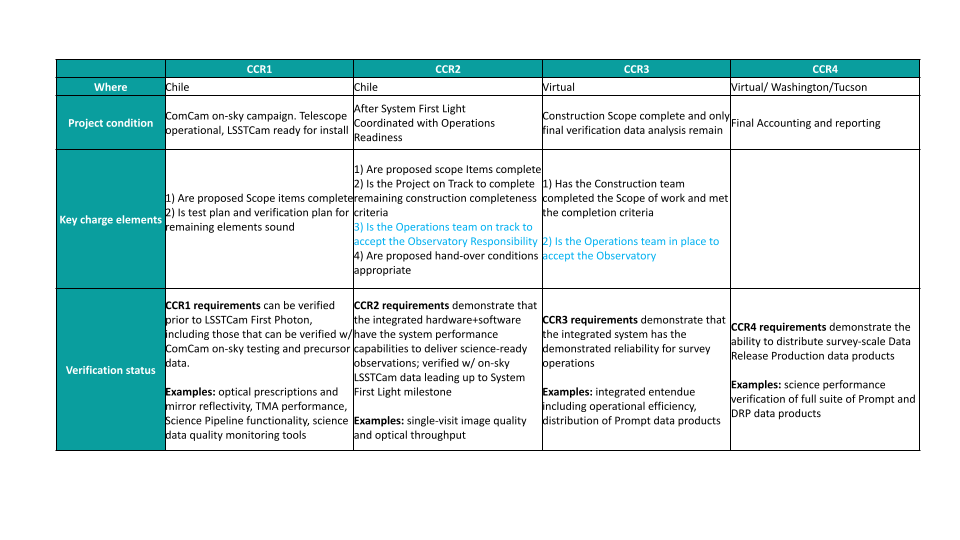
\includegraphics[width=1\textwidth]{./CCRs_overview.png}
    \caption{Construction Closeout Review overview}
    \label{CCRs_overview}
    \end{center}
\end{figure}

The phasing of the four CCRs is intended to clarify the prioritization of activities during the end stages of commissioning, provide opportunities for feedback and iteration with stakeholders regarding the Construction Project deliverables, and coordinate the transition to Operations.
Each of the four CCRs is associated with a different Project condition, as shown by Figure~\ref{CCRs_overview}.
The objectives for each of the four CCRs can be concisely summarized as:

\begin{itemize}

    \item \textbf{CCR1} -- \emph{readiness} for the start of on-sky commissioning, as exemplified by substantial completion and integration of subsystems, and evidenced by direct measurement of the optical throughput of the integrated system

    \item \textbf{CCR2} -- \emph{capability} to support LSST science goals, as exemplified by the System First Light technical milestone, and evidenced by delivered single-visit image quality (including active control of optics)

    \item \textbf{CCR3} -- \emph{reliability} to initiate the LSST survey, as exemplified by Science Validation surveys, and evidenced by the readiness of Rubin Observatory Operations to accept the as-built observatory

    \item \textbf{CCR4} -- \emph{closeout} of the Construction project, as exemplified by service of scientifically validated survey-scale data products as part of the Operations Early Science Program, and evidenced by completed scope of system-level requirement verification, reporting, and final accounting

\end{itemize}